\chapter{МЕТОДЫ УПРАВЛЕНИЯ ЭЛЕКТРОПНЕВМАТИЧЕСКИМ ПРИВОДОМ С ДИСКРЕТНЫМ УПРАВЛЕНИЕМ}\label{ch:ch3}
Управление электропневматическими приводами с дискретными распределителями представляет
собой комплексную задачу, обусловленную нелинейной динамикой пневматических систем и
дискретным характером управляющих воздействий. Эффективное решение данной задачи требует
применения специализированных алгоритмов, способных обеспечить высокую точность позиционирования и
быстродействие системы при ограниченном наборе управляющих состояний. Особый интерес представляет адаптация
классических методов управления к специфике дискретных пневматических систем.

В рамках настоящего исследования рассматривается широкий спектр подходов к управлению электропневматическими
приводами, включающий как современные адаптивные методы, так и модифицированные
классические алгоритмы. Исследуются скользящее управление, прогнозное управление,
нечеткое управление, нейросетевое управление, а также применение широтно-импульсной модуляции (ШИМ)
в сочетании с классическими регуляторами, такими как ПИД-регулятор и его модификации.
Выбор данных методов обусловлен необходимостью комплексного анализа возможностей оптимизации управления
с учетом специфики дискретных пневматических систем. Каждый из рассматриваемых подходов обладает
уникальными преимуществами и ограничениями, детальное изучение которых позволит сформировать
всестороннее представление о перспективах совершенствования алгоритмов управления
электропневматическими приводами с дискретными распределителями.

\section{ШИМ управление с использование ПИД регулятора}\label{sec:ch3/sec1}

\subsection{Принципы реализации ШИМ в пневматических системах с дискретным управлением}\label{subsec:ch3/sec1/sub1}
Широтно-импульсная модуляция (ШИМ) представляет собой метод формирования квазинепрерывного
управляющего воздействия в системах с дискретными исполнительными элементами.
В контексте пневматических систем с дискретными распределителями применение ШИМ
позволяет преодолеть ограничения, связанные с бинарным характером управления, и обеспечить более
точное регулирование положения и скорости исполнительного механизма.

Механизм формирования квазинепрерывного управляющего воздействия
посредством ШИМ основан на периодическом переключении дискретных
распределителей с определенной частотой и скважностью.

Математически это может быть описано следующим образом:

\begin{equation*}
    u(t) = \begin{cases}
        1, & 0 \leq t < \alpha T \\
        0, & \alpha T \leq t < T
    \end{cases}
\end{equation*}
где $u(t)$ -- управляющий сигнал;
$T$ -- период ШИМ;
$\alpha$ -- коэффициент заполнения $0 \leq \alpha \leq 1$.

На рисунке \ref{fig:ch3:pwm_example} показаны временные диаграммы ШИМ-сигнала
с различными значениями коэффициента заполнения.

\begin{figure}[ht]
    \centerfloat{
        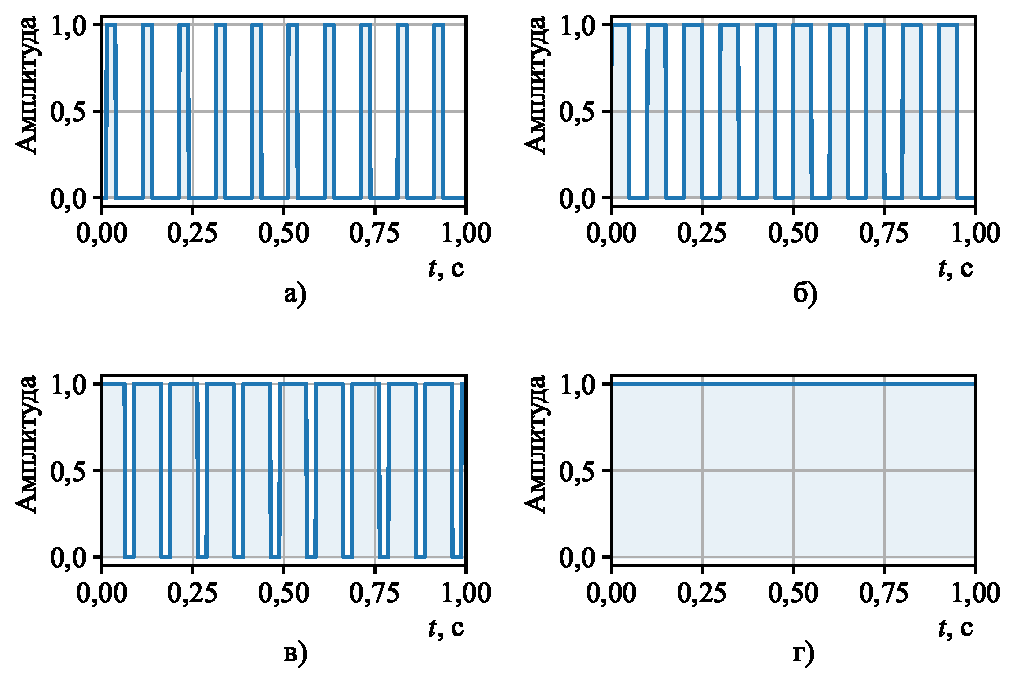
\includegraphics[]{part3/pwm_signal_skewness.pdf}
    }
    \caption{Примеры ШИМ-сигнала с различными значениями коэффициента заполнения}
    \label{fig:ch3:pwm_example}
\end{figure}

Среднее значение управляющего воздействия за период определяется как:
\begin{equation*}
    \bar{u} = \frac{1}{T} \int_0^T u(t) dt = \alpha,
\end{equation*}

Влияние частоты ШИМ на динамику пневмопривода является критическим фактором при
проектировании системы управления. С увеличением частоты ШИМ улучшается
гладкость управляющего воздействия, что способствует снижению пульсаций давления
и повышению точности позиционирования. Однако чрезмерно высокая частота может привести
к повышенному износу распределителей и увеличению энергопотребления.

На рисунке \ref{fig:ch3:pwm_pressure_response} представлены графики изменения
давления в пневмоцилиндре при различных частотах ШИМ.

\begin{figure}[ht]
    \centerfloat{
        % \includegraphics[]{part3/pwm_pressure_response.pdf}
    }
    \caption{Влияние частоты ШИМ на пульсации давления в пневмоцилиндре}
    \label{fig:ch3:pwm_pressure_response}
\end{figure}

Для анализа влияния частоты ШИМ на динамику системы может быть использована передаточная функция эквивалентного непрерывного звена:
\begin{equation*}
    W_{\text{ШИМ}}(s) = \frac{1 - e^{-sT}}{sT},
\end{equation*}
где $s$ -- комплексная переменная преобразования Лапласа.
Особенности применения ШИМ для различных типов дискретных
распределителей обусловлены их конструктивными характеристиками и
динамическими свойствами. На рисунке \ref{fig:ch3:pwm_valve_response} показаны
характеристики переходных процессов для распределителей с различным быстродействием.

\begin{figure}[ht]
    \centerfloat{
        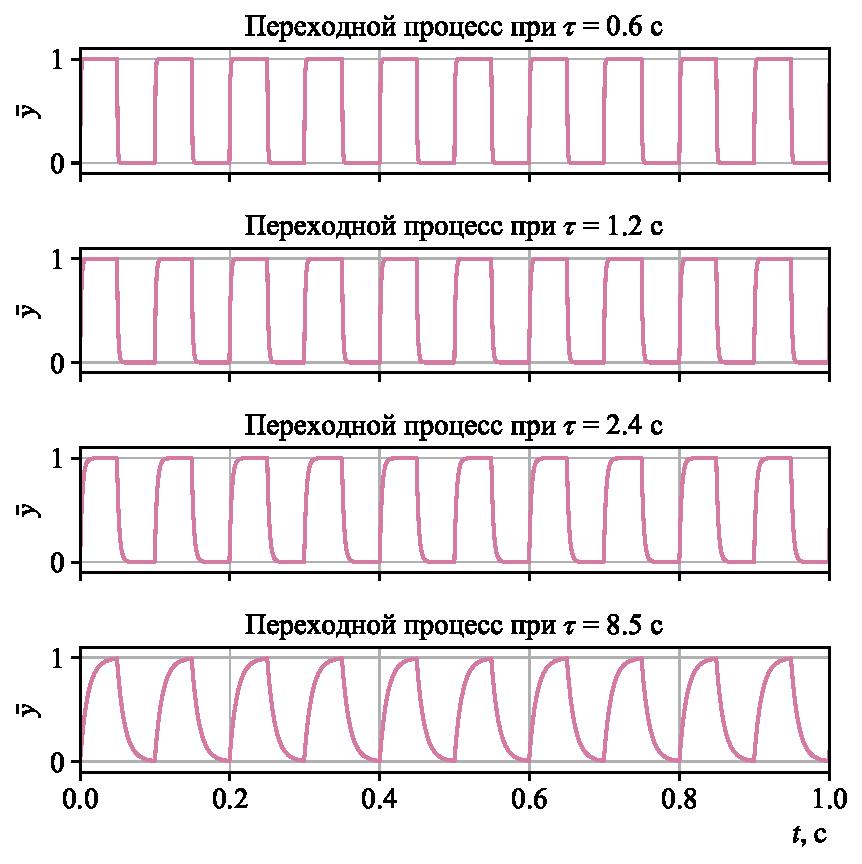
\includegraphics[]{part3/pwm_valve_response.pdf}
    }
    \caption{Характеристики переходных процессов для различных типов дискретных распределителей}
    \label{fig:ch3:pwm_valve_response}
\end{figure}

При выборе параметров ШИМ необходимо учитывать соотношение между
периодом ШИМ и динамическими характеристиками распределителя:
\begin{equation*}
T_{ШИМ} \geq k\tau_{\text{р}},
\end{equation*}
где $\tau_{\text{р}}$ -- время реакции распределителя;
$k$ -- коэффициент запаса (обычно $k \geq 2$).

\subsection{Реализация ПИД-регулирования для пневмоприводов с дискретными распределителями}\label{subsec:ch3/sec1/sub2}
Применение ШИМ в пневмоприводах с дискретными распределителями открывает
возможность использования алгоритмов управления,
изначально разработанных для непрерывных систем.
Одним из наиболее эффективных и широко применяемых методов является
пропорционально-интегрально-дифференциальное (ПИД) регулирование.

Структура ПИД-регулятора для пневмопривода
с дискретными распределителями может быть представлена следующей схемой:
\begin{figure}[ht]
   \centerfloat{
    %    \includegraphics[]{part3/pid_pwn_control.pdf}
    \caption{Структурная схема ПИД-регулятора с ШИМ управлением}
    \label{fig:ch3:pid_pwm_control}
\end{figure}
В данной схеме выходной сигнал ПИД-регулятора преобразуется в коэффициент
заполнения ШИМ, который управляет дискретными распределителями
пневмопривода. Этот подход позволяет достичь высокой точности
управления, характерной для непрерывных систем, в условиях
дискретного исполнительного механизма.

Математическая модель ПИД-регулятора в дискретной форме описывается уравнением:
\begin{equation*}
u[k] = K_p e[k] + K_i T_s \sum_{i=0}^k e[i] + K_d \frac{e[k] - e[k-1]}{T_s},
\end{equation*}
где
$u[k]$ -- управляющий сигнал на k-ом шаге;
$e[k]$ -- ошибка регулирования на k-ом шаге;
$K_p$, $K_i$, $K_d$ -- коэффициенты пропорциональной, интегральной и
дифференциальной составляющих соответственно;
$T_s$ -- период дискретизации.

Выходной сигнал ПИД-регулятора преобразуется в коэффициент заполнения ШИМ согласно формуле:
\begin{equation*}
\alpha = \frac{u[k] + u_{max}}{2u_{max}},
\end{equation*}
где $u_{max}$ -- максимальное значение управляющего сигнала.

\subsection{Модифицированные структуры ПИД регулятора}\label{subsec:ch3/sec1/sub3}
\subsection{Применение усреднителя Смита для компенсации запаздывания}\label{subsec:ch3/sec1/sub4}
\subsection{Каскадные и комбинированные структуры ПИД регуляторов}\label{subsec:ch3/sec1/sub5}
\subsection{Математическое описание и анализ динамических характеристик}\label{subsec:ch3/sec1/sub6}

\section{Управление в скользящих режимах}\label{sec:ch3/sec2}

\section{Нечеткое управление}\label{sec:ch3/sec3}

\section{Прогнозное управление}\label{sec:ch3/sec4}
